\documentclass[letterpaper,9pt,twoside,printwatermark=false]{pinp}

%% Some pieces required from the pandoc template
\providecommand{\tightlist}{%
  \setlength{\itemsep}{0pt}\setlength{\parskip}{0pt}}

% Use the lineno option to display guide line numbers if required.
% Note that the use of elements such as single-column equations
% may affect the guide line number alignment.

\usepackage[T1]{fontenc}
\usepackage[utf8]{inputenc}

% The geometry package layout settings need to be set here...
\geometry{layoutsize={0.95588\paperwidth,0.98864\paperheight},%
          layouthoffset=0.02206\paperwidth,%
		  layoutvoffset=0.00568\paperheight}

\definecolor{pinpblue}{HTML}{185FAF}  % imagecolorpicker on blue for new R logo
\definecolor{pnasbluetext}{RGB}{101,0,0} %



\title{DALITE Q2 - Boxplots, Standard Deviation and Normal Curves Solutions.}

\author[a]{EPIB607 - Inferential Statistics}

  \affil[a]{Fall 2018, McGill University}

\setcounter{secnumdepth}{5}

% Please give the surname of the lead author for the running footer
\leadauthor{Bhatnagar and Hanley}

% Keywords are not mandatory, but authors are strongly encouraged to provide them. If provided, please include two to five keywords, separated by the pipe symbol, e.g:
 \keywords{  Boxplots |  Standard deviation |  Normal curves  }  

\begin{abstract}
This DALITE quiz will cover more descriptives such as boxplots, standard
deviation, and introduce you to normal density curves.
\end{abstract}

\dates{This version was compiled on \today} 

% initially we use doi so keep for backwards compatibility
\doifooter{\url{https://sahirbhatnagar.com/EPIB607/}}
% new name is doi_footer

\pinpfootercontents{DALITE Q2 due Sepetember 19, 2018 by 5pm}

\begin{document}

% Optional adjustment to line up main text (after abstract) of first page with line numbers, when using both lineno and twocolumn options.
% You should only change this length when you've finalised the article contents.
\verticaladjustment{-2pt}

\maketitle
\thispagestyle{firststyle}
\ifthenelse{\boolean{shortarticle}}{\ifthenelse{\boolean{singlecolumn}}{\abscontentformatted}{\abscontent}}{}

% If your first paragraph (i.e. with the \dropcap) contains a list environment (quote, quotation, theorem, definition, enumerate, itemize...), the line after the list may have some extra indentation. If this is the case, add \parshape=0 to the end of the list environment.


\hypertarget{boxplot-properties-q1}{%
\section{Boxplot properties Q1}\label{boxplot-properties-q1}}

A boxplot can show whether a data set is:

\begin{enumerate}
\def\labelenumi{\alph{enumi})}
\tightlist
\item
  symmetric
\item
  skewed
\item
  \textbf{symmetric and skewed (Correct)}
\end{enumerate}

\hypertarget{correct-rationales}{%
\subsection{Correct rationales}\label{correct-rationales}}

\begin{itemize}
\tightlist
\item
  When the data is skewed, the box will be shifted towards one of the
  whiskers (maximum or minimum). Symmetric data will have a median that
  splits the box in half.
\item
  If the data set is skewed, the median locates above or below the
  center of the box plot, and the box locates closer to the maximum or
  minimum values.
\end{itemize}

\hypertarget{incorrect-rationales}{%
\subsection{Incorrect rationales}\label{incorrect-rationales}}

\begin{itemize}
\tightlist
\item
  A boxplot can show the mean, quartiles which can tell us about being
  symmetric
\item
  Mean, quartiles, and the max/min values in the plot help to show the
  symmetry and skewness of the data
\end{itemize}

\hypertarget{boxplot-properties-q2}{%
\section{Boxplot properties Q2}\label{boxplot-properties-q2}}

If one side of the box is longer than the other, it means that side
contains more data.

\begin{enumerate}
\def\labelenumi{\alph{enumi})}
\tightlist
\item
  TRUE
\item
  \textbf{FALSE (Correct)}
\end{enumerate}

\hypertarget{correct-rationales-1}{%
\subsection{Correct rationales}\label{correct-rationales-1}}

\begin{itemize}
\tightlist
\item
  The box is created by first finding the median which is the value half
  way between your ordered data. The quartiles are found by taking the
  medians of the upper and lower half of your data. Therefore, each
  quartile or side of the box contains the same amount of data it is
  just that if one side has larger values it will cause the boxplot to
  be skewed, making the box appear longer on one side.
\item
  There is the same amount of data/observations in each quartile. The
  size of the quartiles is an indication of the spread of the
  observations within that quartile.
\end{itemize}

\hypertarget{incorrect-rationales-1}{%
\subsection{Incorrect rationales}\label{incorrect-rationales-1}}

\begin{itemize}
\tightlist
\item
  The quartiles represent the number of data located within 25\%, 50\%
  75\% positions. Therefore the longer the box, the greater the number
  of data located within that percentile
\end{itemize}

\hypertarget{boxplot-properties-q3}{%
\section{Boxplot properties Q3}\label{boxplot-properties-q3}}

The figure below shows histograms from two different data sets, each one
containing 18 values that vary from 1 to 6. The histogram on the left
has an equal number of values in each group, and the one on the right
has two peaks at 2 and 5. Which of the following statements is true?

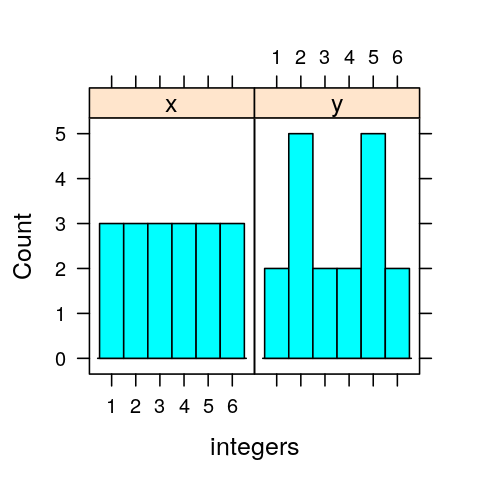
\includegraphics{hist.png}

\begin{enumerate}
\def\labelenumi{\alph{enumi})}
\tightlist
\item
  The boxplots for each histogram will be different.
\item
  \textbf{The boxplots for each histogram will be the same (Correct)}
\item
  There is not enough information to tell us if the boxplots will be the
  same or if they will be different.
\end{enumerate}

\hypertarget{correct-rationales-2}{%
\subsection{Correct rationales}\label{correct-rationales-2}}

\begin{itemize}
\tightlist
\item
  They will be the same because the 5 summary statistics (min, Q1,
  median, Q3, and max) will be the same and thus, both boxplots will be
  visually identical.
\item
  Both histograms are symmetric therefore the boxplots will be the same
  and won't difference in data distribution
\end{itemize}

\hypertarget{incorrect-rationales-2}{%
\subsection{Incorrect rationales}\label{incorrect-rationales-2}}

\begin{itemize}
\tightlist
\item
  In the first histogram the values are equal which would create a very
  symmetric boxplot. Whereas in the second histogram, there are two
  counts which are higher than the rest and that would produce a more
  uneven boxplot.
\item
  Although the median for both distributions is the same, the spread
  around the median differs, and this would account for differences in
  quartiles and therefore the shape of the boxplots
\end{itemize}

\hypertarget{question-standard-deviations-q1}{%
\section{Question : Standard Deviations
Q1}\label{question-standard-deviations-q1}}

Researcher 1 takes a sample of 100 men age 18-24 in a certain town. In
the same town, Researcher 2 takes a sample of 1000 men age 18-24. Which
of the following statements is true?

\begin{enumerate}
\def\labelenumi{\alph{enumi})}
\tightlist
\item
  The average height for the sample collected by Researcher 2 will be
  bigger than the average height for the sample collected by Researcher
  1
\item
  The standard deviation of heights for the sample collected by
  Researcher 2 will be smaller than the standard deviation of heights
  for the sample collected by Researcher 1
\item
  The sample collected by Researcher 1 will likely contain the tallest
  of the 1,100 men.
\item
  \textbf{The sample collected by Researcher 2 will likely contain the
  shortest of the 1,100 men. (Correct)}
\end{enumerate}

\hypertarget{correct-rationales-3}{%
\subsection{Correct rationales}\label{correct-rationales-3}}

\begin{itemize}
\tightlist
\item
  Because Researcher 2 is sampling from more of the population he/she
  more likely to include the shortest and tallest of the population.
\item
  this is true because having a bigger sample may allow greater
  inclusion of the outliers
\item
  Over 90\% of the population will be captured by Researcher 2, so the
  sample will likely contain the shortest of the men. Standard deviation
  will not necessarily be smaller because it is the SD of the sample,
  not of the sample means.
\end{itemize}

\hypertarget{incorrect-rationales-3}{%
\subsection{Incorrect rationales}\label{incorrect-rationales-3}}

\begin{itemize}
\tightlist
\item
  Since sample size is the denominator to calculate standard deviation,
  a larger sample size will yield a smaller standard deviation.
\item
  Because as you increase the sample size, you get the same or similar
  values more often.
\item
  Assuming that heights are relatively normally distributed, collecting
  more samples would reduce the spread of their distribution (this can
  be visualized in the formula - when n increases, s decreases)
\end{itemize}

\[
\sigma^2 = \frac{1}{n} \sum_{i=1}^n (x_i - \bar{x})^2
\]

\hypertarget{standard-deviations-q2}{%
\section{Standard Deviations Q2}\label{standard-deviations-q2}}

If you add 7 to each entry on a list of numbers (which contains both
positive and negative integers), that adds 7 to the standard deviation.

\begin{enumerate}
\def\labelenumi{\alph{enumi})}
\tightlist
\item
  TRUE
\item
  \textbf{FALSE (Correct)}
\end{enumerate}

\hypertarget{correct-rationales-4}{%
\subsection{Correct rationales}\label{correct-rationales-4}}

\begin{itemize}
\tightlist
\item
  Adding a constant, 7, to all data values shifts the location of the
  data but does not affect its spread. -In the numerator of the formula
  for standard deviation, the added 7s would cancel out:
\end{itemize}

\[((x+7)-(\bar{x}+7))^2 = (x-\bar{x})^2\]

\hypertarget{incorrect-rationales-4}{%
\subsection{Incorrect rationales}\label{incorrect-rationales-4}}

\hypertarget{normal-curves-q1}{%
\section{Normal Curves Q1}\label{normal-curves-q1}}

To completely specify the shape of a normal distribution, you must give:

\begin{enumerate}
\def\labelenumi{\alph{enumi})}
\tightlist
\item
  the mean and standard deviation (Correct)
\item
  the five-number summary (min, Q1, median, Q3, max)
\item
  the mean and the median
\item
  the mean and the interquartile range
\end{enumerate}

\hypertarget{correct-rationales-5}{%
\subsection{Correct rationales}\label{correct-rationales-5}}

\begin{itemize}
\tightlist
\item
  This is a basic characteristic of normal distributions. If normal,
  they all have predictable properties and allow us to understand a
  great deal about them with these two values.
\end{itemize}

\hypertarget{incorrect-rationales-5}{%
\subsection{Incorrect rationales}\label{incorrect-rationales-5}}

\hypertarget{normal-curves-q2}{%
\section{Normal Curves Q2}\label{normal-curves-q2}}

Which of the following statements is false regarding normal curves?

\begin{enumerate}
\def\labelenumi{\alph{enumi})}
\tightlist
\item
  the mean of a normal density curve shifts the curve along the
  horizontal axis without changing its shape
\item
  increasing the standard deviation produces a flatter and wider
  bell-shaped curve and that decreasing the standard deviation produces
  a taller and narrower curve
\item
  area under a density curve over an interval represents the proportion
  of data that falls in that interval
\item
  \textbf{unlike the average, the standard deviation is not sensitive to
  outliers. (Correct)}
\end{enumerate}

\hypertarget{correct-rationales-6}{%
\subsection{Correct rationales}\label{correct-rationales-6}}

\begin{itemize}
\tightlist
\item
  The standard deviation is a measure of spread, if you have outliers,
  your data is more spread, thus increasing your standard deviation.
\end{itemize}

\hypertarget{incorrect-rationales-6}{%
\subsection{Incorrect rationales}\label{incorrect-rationales-6}}

%\showmatmethods


\bibliography{pinp}
\bibliographystyle{jss}



\end{document}

